\documentclass{article}
\usepackage[utf8]{inputenc}
\usepackage{graphicx}
\usepackage{subcaption} 
\usepackage[export]{adjustbox}

% change reference style to [1], remove stupid sorting, language changed so date in ddmmyyyy
\usepackage[backend=biber, style=numeric, sorting=none, language=australian]{biblatex}
\addbibresource{References.bib}

\title{Dissertation - Detecting User Engagement Using Mouse Tracking Data}
\author{David Saunders (910995)}
\date{September 2020}

\begin{document}
\maketitle

\begin{abstract} 
    %Potential abstract.
    This project explores the use of Hidden Markov Models to explore users mouse cursor data while performing a task.
    The users are split into 2 distinct groups, online crowdsourced users, and lab study users.
    We propose that the lab study users were paying attention, and the crowdsourced users may or may not be paying attention.
    By using observed data recorded from the users mouse we are able to model both groups interaction with the system with Hidden Markov Models.
    Some users interaction seem misplaced compared to their groups.
    These are reclassified with the aim of changing the groups of user from lab study or crowdsourced, to users paying attention and not paying attention.     
    It was found that 26\% turk users were paying attention, and 20\% of lab study users were not paying attention.
    These results require further research with a properly labelled dataset to confirm any findings.

\end{abstract}

\tableofcontents

% Toms layout

% Motivation
% Related Work
% Implementation
% Results
% Conclusion

\section{Motivation}

% Why is it important
% Why is it a hard problem/problems
% Why other authors have failed
% My contributions are - bullet list
% My idea to fix it

% Original before copying from project specification

% Detecting use engagement is an important science across multiple disciplines.

% Find a study that says during any task / any crowdsourced task X\% of people are not paying attention.
% This could jeopardise the results from any online if we cannot be sure users are actually paying attention to the task they are being paid to complete. 

% It is a hard problem because, among other things I will touch on, it is hard to quantify exactly what user engagement is exactly.
% One author defined it as 'XYZ' [look at my previous work for references].

% However the previous authors have failed to detect and measure user engagement as X,Y,Z.


% TODO talk about some of the papers Tom links in his paper, such as  
% Finding Waldo: Learning about users from their interactions
% His paper literally outlines my project so defo worth exploring what he says.

% COPIED DIRECTLY FROM PROJECT SPECIFICATION

%https://academia.stackexchange.com/questions/44784/how-to-explain-things-in-the-motivation-section-of-a-mathematical-paper-without
% People have wondered about how to better understand frobs ever 
% since Richard Feynman first used them to pick the locks in Los Alamos. 
% Although X, Y, and Z attempts have been made, none of them got very far
%  because they were all green-colored. 
%  In this dissertation, I examine an alternate path, reducing the problem
%   of frobs to the simpler system of greebit-space by means of an 
%   innovative application of wibbling. 
%   These results bring us one step closer to solving the problem of frobs, 
%   and how they can be better used to quickly and cheaply pick locks.

% Paragraph 1 - Initial motovation
Crowd-sourcing marketplaces like Amazon’s Mechanical Turk are popular services that provide a method for researchers to get participants to complete human intelligence tasks \cite{paolacci2010running}. 
A common use for this technology is to label data for use in training for machine learning algorithms \cite{chang2017revolt}.
However, they can also provide a cheap, scalable method for scientists to gather responses in research.
The level of user engagement, attention, and low quality responses can all be issues when gathering data from participants with distributed approaches \cite{ipeirotis2010quality}.
The primary motivation of this project is to develop a system of potentially identifying if a crowdsourced user is paying attention during a task.

% Paragraph 2 - Inter disciplinary
The use of gathering responses using Amazon's Mechanical Turk and other crowdsourcing alternatives are becoming prevalent across disciplines.
It is commonly used in conducting clinical research \cite{chandler2016conducting} and it is estimated that almost half of all cognitive science research involves the use of crowdsourcing services to collect data samples \cite{stewart2017crowdsourcing}.
The creation of an easy to implement method to measure user engagement would massively help researchers to increase reliability of their research.

% Paragraph 3 - Motivation
Research has been conducted on how the accuracy and attention of crowdsourced tasks can be increased.
% Look at these papers to see how they classified attentions.
Methods such as offering financial incentives \cite{ho2015incentivizing} and engaging a users curiosity \cite{law2016curiosity} have been found to motivate workers into performing better at crowdsourced tasks.
Despite the research there is still debate as to which method is superior.
If user engagement can be effectively identified then the best method of ensuring user engagement could be found using this method.

% Paragraph 4 - Why measuring attention is hard and why obvious solutions wont work. 
% It's worth spending some space on why this problem is hard and why any obvious solutions won't work

%Maybe it is hard to quantify attention as it is hard to do so.
%Measuring attention is hard and obvious solutions wont work.
Measuring user engagement is well studied in the field of web analytics \cite{peterson2008measuring}.
However the existing methods of reporting and analysing website data cannot be easily applied to crowdsourced tasks.    
Characteristics such as session duration and customer satisfaction are used as proxies for engagement.
However a longer session doesn't necessarily mean a more engagement user and customer satisfaction is not applicable for crowdsourced tasks.
Therefore existing solutions will not work and now methods must be evolved.


\subsection{Background}
% TODO Find the Gruber thesis and the paper written by Tom.

% TODO Have this section finished soon and have Meg look over it: 04/09/20

The work in this project is build on an existing study;
\textit{``Risk fixers and sweet spotters: A study of the different approaches
to using visual sensitivity analysis in an investment scenario''}\cite{torsney2018risk}.

The study was centred in the field of visualisation.
The paper explored a new visualisation glyph that could be used help improve a users effectiveness at completing a task.
The users task simulated an investment scenario, the aim was to maximise the return of a collection of stocks, while minimising the risk. 

\begin{figure}[ht]
    \centering
    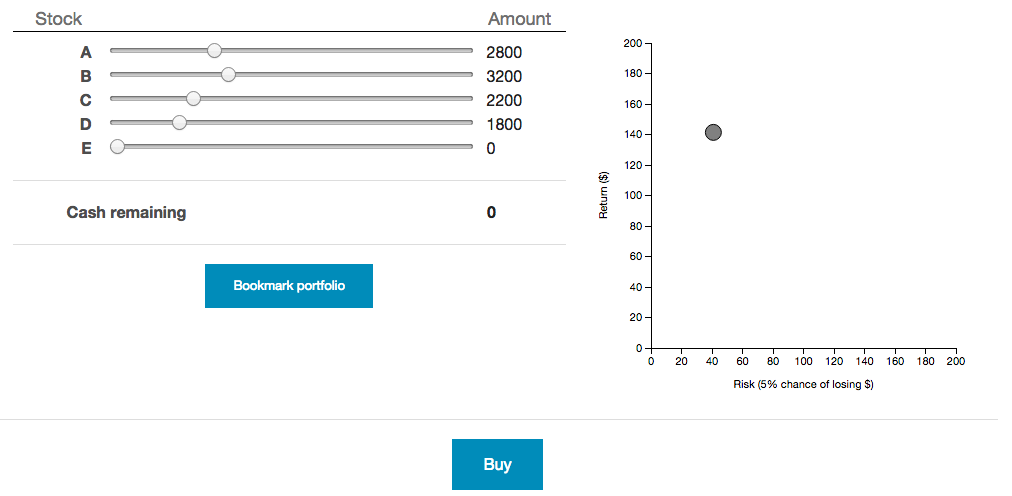
\includegraphics[scale=0.3, frame]{Images/interface.png}
    % TODO: Find the right interface, current interface doesn't match whats in his paper.
    \caption{The user interface of the lab study, showing the risk and return of stocks to the left and allocation sliders to the right.}
    \label{fig:interface}
\end{figure}

The experiment identified two users groups, risk fixers and sweet spotters, based on their response in a questionnaire.
Figure \ref{fig:interface} shows the interface of the lab study.

We divided the participants based on their response to a question
about how they chose their final portfolio. 


\begin{table}[ht]
    \caption{\label{table:studies} Data collection methods used in the study \cite{torsney2018risk}.}
    \small
    \begin{tabular}{lll}
        \hline
        Data collection method & Number of participants & Were participants paying attention? \\    \hline
        Lab study              & 18                     & Yes                                 \\
        Crowdsourced task      & 370                    & Unknown                             \\    \hline
    \end{tabular}
\end{table}

Table \ref{table:studies} shows the two different ways in which data was collected.
Only 4.6\% of the data was gathered in person, with the vast majority of responses being crowdsourced.
The difference in number of participants shows one of the reasons crowdsourcing is popular. 
It is much easier to crowdsource responses than it is to organise an in person lab study.


\subsection{Initial attempt}

One naive assumption might be that a users attention level might be inferred from the time taken to complete the tasks.
Exploration of the data showed that the division of users may not be so straightforward, shown in Figure~\ref{fig:scatterplot}.
% TODO add plot of lengths vs time for different groups.

\begin{figure}[ht]
    \centering
    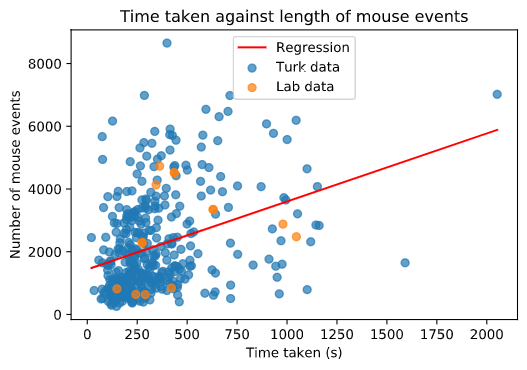
\includegraphics[scale=0.6]{Images/TimeTaken-Mouse-Events.png}
    % TODO: Find the right interface, current interface doesn't match whats in his paper.
    \caption{Scatterplot of users.}
    \label{fig:scatterplot}
\end{figure}

The lab and turk user classes cannot be separated by a simple metric of their data, such as length of events sequence and time to complete task.
This rules out distance based machine learning approaches such as K Nearest Neighbours or a Support Vector Machine as there is no relationship there.
It should be noted that length of events sequence and time are correlated with a pearson's correlation of $0.344$.

As a rule of thumb we can say that correlations below 0.3 have no relationship, and values between 0.3 and 0.5 have a weak relationship \cite{mindrila2017scatterplots}.
This means the 2 features are weakly correlated, but correlated nonetheless.
This means that one of these features may be a good substitute for the other and that having both may be redundant.

\subsection{Contributions}
% The contributions are 1,2,3 (everyone likes 3s)
% Take aways of how it will help them.

In this project my contributions to fix it are, -a system to classify users, a way of visualising their mouse paths, ways to directly and quantitatively compare different users, and a multistage semi-supervised based binary classification output to answer the question of 'are users engaged'.

\section{Related Work}

% Convince the reader you've done enough work and research in the area.
% Convince them it was hard and the topic is hard so you need to help.
% You've tried other peoples techniques.

All related work about actual other attempts to detect user engagement from mouse tracking data.
Other subsections will be like miniature literature reviews or something?

% Taken from project specification

% Dont really link to engagement 
\subsection{Eye tracking}

Non-verbal information such as eye tracking may be used to detect user’s level of engagement \cite{lala2017detection}.
Vision is one of the most powerful human senses so it has the potential to give a good measure of user engagement. 
The methodology of eye tracking is that we move our eyes to focus on particular areas that we want to see in more detail, and divert our attention to that area \cite{duchowski2007eye}. 
% duchowski2007eye is a VERY important piece of literature for the field, over 4000 citations
Thus tracking a user’s gaze can provide insight into which part of a system they’re engaged with, and how much so.

\begin{figure}[ht!]
    \centering
    \centerline{
        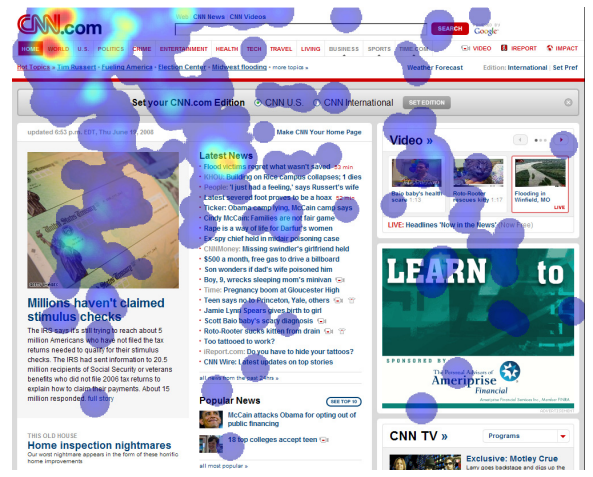
\includegraphics[scale=0.7]{Images/EyeHeatmap.PNG}
    }
    \caption{Heatmap showing popular locations of users eyes on a webpage \cite{buscher2009you}.}
    \label{fig:eyetrack}
\end{figure}

Eye tracking data can be used to show user interface elements that users focus their attention on as shown in Fig \ref{fig:eyetrack}. 
From this researchers were able to predict the amount of attention elements of the page would receive.
By observing what parts of an interface users are interacting with we can determine what a user is engaging with \cite{buscher2009you}.
Eye-tracking has been used, and found success novel applications such as recording the engagement of users when playing a game. 
Tracking users eye movements helped game designers understand how users can recognise interactable game objects and could be used to investigate problematic game design issues \cite{renshaw2009towards}.

Eivazi and Bednarik extracted features from a users eye tracking data to determine their cognitive state in a problem solving exercise \cite{eivazi2011predicting}.
Features such as ``mean fixation duration'' and ``total path distances'' were engineered, and users were split into classes based on their performance. 
Given a user feature set and their performance class it was able to classify their cognitive state during the task with a 87.5\% accuracy with a support vector machine.

Szafir and Mutlu identified a plethora of verbal and non-verbal behavioural cues used by teachers in an educational setting, with gaze being identified as one of them \cite{szafir2012pay}.
The behavioural cues could not be recorded directly by a computer, instead EEG signals measured from a headset were used to measure engagement.

Eye tracking is not however a perfect solution and its limitations have been well documented. 
Track subjects eyes with a good degree of accuracy requires the use of expensive, intrusive equipment that frequently needed recalibrating \cite{richardson2004eye}. 


\subsection{Mouse cursor tracking}
% Copied straight from CSCM10 Initial Report
% Mouse cursor tracking

Research has also found that there is a correlation between a user’s gaze and their cursor position. 
The position can be considered a ``poor man’s eye tracker'' as it has been found that eye gaze match mouse position 69\% of the time \cite{cooke2006mouse}. 
Mouse movement data can be collected without the drawbacks of eye tracking and with more automatic methods, meaning more data can be collected, and on a larger scale \cite{demvsar2017quantifying}.
Therefore it can be said that mouse data can be used as a good alternative to eye tracking data.

%Mouse activity can be used as input to a neural network and output a quantifiable level of activity for a webpage. 
By using mouse data it is possible to unobtrusively record a user’s normal use of a web browser without disturbing their experience \cite{goecks2000learning}.
% Above paper touches on one of the big advantages of measuring user engagement from mouse data, it is unobtrusive! We can monitior them in the background 
It has also been found that users tend to follow the text they are reading with the mouse cursor \cite{liu2007detecting}. 
It can be determine what paragraph of a page was being read with an accuracy of 79\% by using mouse cursor data \cite{hauger2011using}. 

Other methodologies explored ways of classifying user engagement from eye and cursor data, however it is also possible to predict users attention and user frustration in complex webpages \cite{navalpakkam2012mouse}.
Not all studies agree that mouse cursor is always a good approximation for eye data. 
Hauger et al found that distinct cursor behaviour exists depending on the task, and that the relationship between eye gaze and mouse position is more nuanced than measuring only mouse data \cite{huang2012user}.

% \subsection{Machine learning techniques}
% I've given a high level overview of the existing literature, here I will be more in depth as to the algorithms and techniques relevant to this project.

% these subsections below are old
% probably pointless as theyre just some ML techniques and not backgroud

\subsection{Semi Supervised Learning}
This will be a key aspect of the project as we only have definitive labels for part of our data.
This reflects the challenges of real world data, by some estimates only 2\% (made up number) of all data is structured and labelled, the rest is unstructured [find reference].

In a sense the data here is labelled.
All day belongs to 2 classes, online turk user, or in person lab study user.
However on the other hand the data is not labelled for the task I would like to explore.
The goal of this project is to identity which users were paying attention.
We have assumed that we can infer that lab study users will be paying attention, so we can say that those samples are labelled.
However the rest of the samples we have which are all of the online data are unlabelled.
Therefore this is a kind of semi supervised learning problem where we only have a small percentage of our samples labelled, and only confident labels for one class.
(See if a paper on this exists, semi supervised binary classification with only labels for one class.)
% Do a literature review type of thing where I review semi supervised learning, talk about methods and how they can be applied to what I'm trying to do.

\subsection{N-Grams}
This paper has a nice scientific explanation of n-grams \cite{tomovic2006n}.
Either cite this paper or more likely look at their reference for n-grams and cite that.

\subsection{Hidden Markov Models}

% explanation from scratch: https://towardsdatascience.com/hidden-markov-model-implemented-from-scratch-72865bda430e

"Hidden Markov Model (HMM) is a statistical Markov model in which the system being modeled is assumed to be a Markov process – call it X – with unobservable ("hidden") states. 
HMM assumes that there is another process Y whose behaviour "depends" on X.
The goal is to learn about X by observing Y." Wikipedia

In the case of this project, the hidden states X would be the users thought processes including whether or not they're paying attention.
The observations, Y, are the data that has been collected from the users such as mouse location over time and sequence of interface elements.

Paper Tom send me about HMM for text classification that I might be able to use \cite{collins2016tagging}.

Paper claims to use HMM for spam detection, I think they actually just use it to detect misspellings of words or something which is used by spam to hide from filters \cite{gordillo2007hmm}.
Probably could find a better spam detecting HMM, I just like how this almost does something different from the title, which my diss will end up doing.

This paper was recommended by someone on stack overflow as an old influential paper in the field with tens of thousands of references \cite{rabiner1989tutorial}.
Called a tutorial on HMM and its so old so original source. 
Would definitely be good to reference if I include any of the mathematics behind HMMs. 

Someone's dissertation on the topic of generating synthetic data with HMMs.
This can be a good way to create synthetic data \cite{ferrando2018generating}.

Maybe this would belong under implementation?
%HMM-Example-Diagram.png
\begin{figure}[ht]
    \centering
    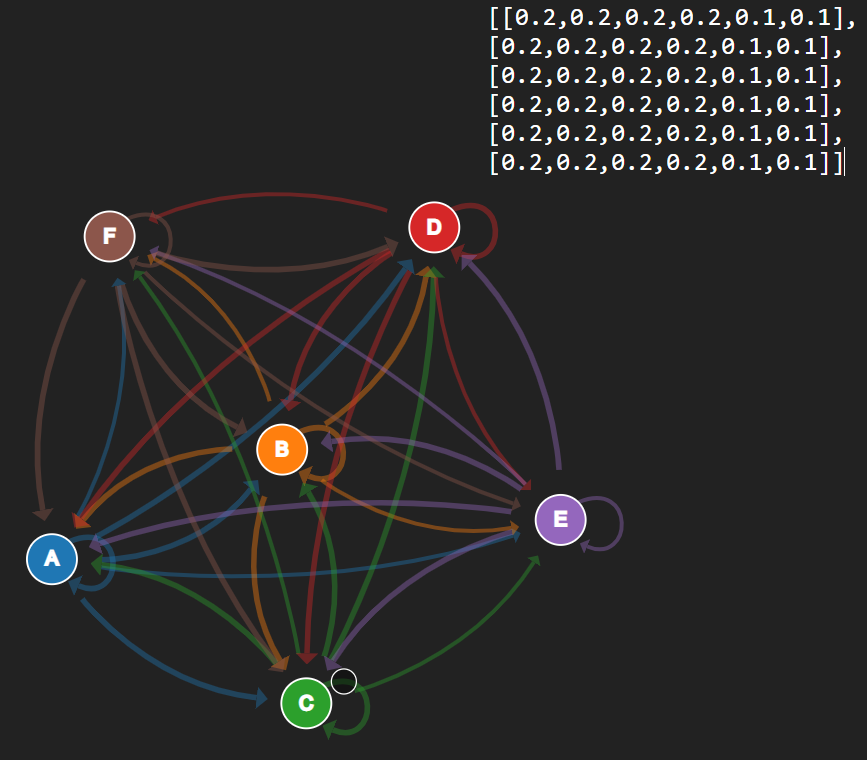
\includegraphics[scale=0.4]{Images/HMM-Example-Diagram.png}
    \caption{Diagram of a Markov Chain model representing a users mouse position}
    \label{fig:Markov}
\end{figure}

Figure \ref{fig:Markov} shows the states of a markov model of my system with states A-E representing sliders 1-5 and state F representing an html element.
In the top right we can see a possible transition matrix of our system.

\section{Implementation}

% Talk about all different steps you took?
To implement a HMM the python library HMMLearn was used \cite{hmmlearn}.
The sequence data used to train the models was the order of mouse targets.
The temporal aspect of the data was ignored, but earlier research showed that number of mouse events and time were heavily correlated.
Therefore using just the order of mouse events should capture the temporal aspect of the data.

When implementing a Hidden Markov model on the actual data there are lots of parameters that must be considered. 
Given a sequence of input data the HMM model can calculate most of the parameters such as the transition matrix by using the Forwards-Backwards algorithm.
The most prominent parameter that must be given is the number of hidden states to use.

The paper \cite{pohle2017selecting} addresses this issue on similar data.
The authors use a HMM to model animal movement behaviour, where they hope the hidden states would roughly relate to the behaviour of the animal.
For example a 2 state HMM on this model may relate to "foraging/resting” and “travelling".
Humans can be more complex than animals but we can think of potential states of being "inquisitive" and "bored"
They trained models with 2, 3, 4, and 5 hidden states and compared the criterion's of AIC, BIC, ICL.
Similarity to evaluate Lab and Turk models models were trained with number of hidden states ranging from 1 to 11.
Generally an increase in states should increase the effectiveness, however it will also take longer to train.
All models used for this comparison was trained to 50 iterations for a fair comparison. 

\begin{figure}[ht]
    \centering
    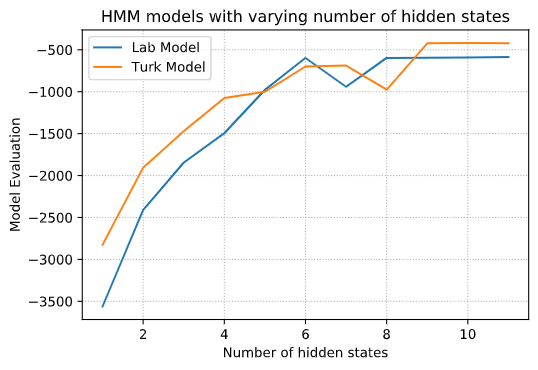
\includegraphics[scale=0.55]{Images/ModelEvaluation.png}
    \caption{Line plot of evaluation of different HMM architectures.}
    \label{fig:ModleEval}
\end{figure}

Figure \ref{fig:ModleEval} shows a different criterion of the total log likelihood of the training data of the model.
This value is normalised by dividing by the number of data samples, to give a per-sample total likelihood.
The evaluation of each HMM model does fluctuate based on the random state used, which is why there are drops in the evaluation criterion even when more hidden states are used.
We can see that the criterion for both models stop improving after 9 states.
Therefore a 10 state model was used.

% https://projecteuclid.org/download/pdfview_1/euclid.aoas/1491616885
% paper A MULTIVARIATE MIXED HIDDEN MARKOV MODEL FOR BLUE WHALE BEHAVIOUR AND RESPONSES TO SOUND EXPOSURE
% interesting reference

\section{Methodology}

%(1/2 page to 1 page)
%(maybe in methodology)
 The assumption of this project is that labs are paying attention and turks are not. Therefore if we get any outliers from the turk data, but that are similar to the lab data, then we will say that that online turk user was paying more attention than his peers, and that they were paying attention.

This study (ref) says that only 10\% of all people / turk users pay attention during a task.
We will look at the 10\% (30ish) of the turk data that looks like it is lab data and day that they were paying attention.
This is just the assumption we have made for the project, 
unfortunately the dataset isn't extensive enough for us to fully test this hypothesis.

\section{Data Pipeline}

When planning and completing this project many decisions were made about the steps taken to convert the raw data to a finished product/classification.
This section may act as an overview of the project, detailing the different sections of work, what they may contain, and the order in which they will be completed.

\begin{figure}[ht]
    \centering
    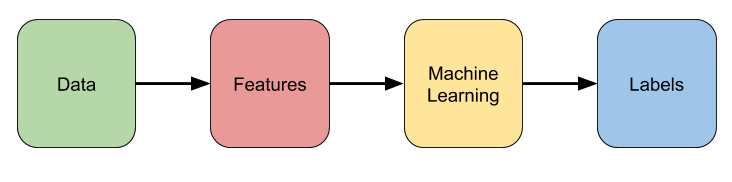
\includegraphics[scale=0.55]{Images/Data-Pipeline.png}
    \caption{Diagram of the Data Pipeline of the project.}
    \label{fig:test}
\end{figure}

% Everyone is a question

\subsection{Data}

% Duplicate or remove to deal with imbalances.
% Probably less effective focusing on this rather than features.

Here I will summarise what I have done to the data.
As previously mentioned the data was gathered through a lab study and an online study.
The purpose of the online study was to gather a larger amount of data that was possible to do so in person.
The aim of this was to make any results more statically significant.
Data was recorded in a big JSON dump with lots of irrelevant and repealed data relating to the users background and not their mouse movements.
Pythons JSON couldn't directly convert the data as mouse events were stored as a nested JSON dictionary and there were errors in the way it was written making it invalid JSON.
Took ages and should explain more indepth, but then finally got data into a tabular data format of a csv which I am more comfortable working with.
Ended up with over 100,000 lines? Might have been more. 

This leads to the problem of imbalanced data samples.
There were approximately 11 lab data and 400 online data, meaning that there were 40x as many data samples from one class compared to the other.
As stated in my assumptions, we can say that the lab participants were paying attention, where as the online participants may or may not have been paying attention.

If the classes were balanced then simple approach may be to treat this problem as binary classification problem.
Using something like a Support Vector Machine we could classify a given point as lab or online / paying attention or possibly paying attention based on their proximity to other data points.
To do so we would need to have balanced classes otherwise the algorithm would have a high accuracy from just classifying everything as possibly paying attention as that is the most frequent class.
There are two main methods of dealing with class imbalances, removing data samples and creating new data samples.

It was decided that creating new data samples would be best as there is not a whole lot of data to work with, so there would be a strong preference to keep the data we have.
New points can be created by sampling from a distribution (reference) but here it was decided just to duplicate the samples as there was no discernible distribution of the data.
Another method is to copy the points, altering them slightly, this was considered but not used in the end.
Each lab study data sample was copied 40 times to even out the classes.

\subsection{Features}

% Tom said something about this being where I should spend the most time of my project.
% Spending time here will be more time effective than other sections.
% This is what people wanna see?
% Evaluating effectiveness of different features.

% What do I so to the raw data.

% What are good features? Big/Good question split into smaller sections.

This part of the pipeline refers to what features I am going to extract from the data.
Features of data can be defined as 'attributes or interesting things from the data'. [reference]
These will consist of both raw and created features, but what do I mean by this?
Raw features will consist of the the number of mouse events recorded, while a created feature could be comparing the trace of users cursor data when using the program.

\subsection{Machine Learning}

% What ML will I do and what algorithm.
% MAybe clustering algorithm but on what data?

Once we have insightful features from the data we can consider what machine learning algorithm would be most appropriate to use on the data.
This will obviously be highly dependent on what form the final features are in.
For example if the features are numerical values such as time taken to complete task and number of mouse events then an algorithm such as a Support Vector Machine would be a good choice.
If the data is in the form of sequential data such as a list of all mouse events then something like a LSTM or RNN network would be best suited.
If the features output was an image such as a trace of mouse position over time then a CNN could be a good choice as they're designed for image data.
It is likely that text classification algorithms will be used when comparing the targets of mouse events.
Comparing n-grams can be done with algorithms such as XYZ [reference].
Other text classification algorithms such as cosine similarity or sentiment analysis could also be used.


\subsection{Labels}

% Who's paying attention

Lastly an important section of the pipeline, as it reflects the final outputs of the system.
Labels will refer to which users are classified as paying attention and which users are not.
A key aspect of this project will be semi-supervised learning.
That is we have some data points we can confirm were paying attention, and others where they're level of attention was questionable.
Once we have an algorithm that can classify some users as paying attention or not we can rerun the algorithm with these preliminary outputs as new training data.
If this is done recursively then we can end up with a system that can split all data points into the 2 classes, perhaps with a degree of confidence given as a percentage.


\section{Repeated Experiments}
% Suggested by Tom as an overview of all the work I've done. 
% Lots of it will probably need adjusting and deleting.

This section will give an overview of the work I have completed during this project.
Each sub section offers a unique approach to tackling the problem.
The different methods were tried sequentially, and the pipeline had to be amended for each one as the input requirements changed.

Approach of this project was to try many different methods of looking through, classifying, and predicting attentiveness of this data.

(Get the actual exploration and ml/data science steps by looking at notebooks.)

\subsection{Distance Based Methods / Spacial Classification Methods}

Not sure if this is the best name for it.
These experiments attempted to separate the data samples for turkers, and lab participants by plotting samples in space.
The aim is that this might reveal information about the features of different users.
If there was a clear distinction between the classes then we could potentially reclassify some points based on their euclidean distance to one another.

\subsubsection{SVM separation methods}
Here we look at if a simple hyperplane could separate the data when looking at similar features the number of mouse events and the total time taken to do the task. 
It was found that a linear, or hyperbolic(wasn't hyperplane was something else) was unable to separate data. 
This was mainly die to the unbalanced classes.

Here simple features of the data was used, the time taken to complete the task, and the number of mouse event taken to complete the task.


\subsubsection{Clustering}
Didn't do this but its an example point.
(Might have tried kNN).

\subsection{Bag-Of-Words Methods}

(Maybe mention bag-of-words models in background research?)

Can treat each target as a word as use NLP methods such as bag-of-words. 
With with method we will lose data regarding order but that can be analysed later with HMMs.
"In this model, a text (such as a sentence or a document) is represented as the bag (multiset) of its words,
 disregarding grammar and even word order but keeping multiplicity.
  The bag-of-words model has also been used for computer vision." 
  - ($wikipedia.org/wiki/Bag-of-words_model$)

Disregarding grammar is a big weakness of traditional uses of BoW but the concept of grammar is meaningless in the case of a sequence of mouse targets.

\subsubsection{Naive Bayes}

Another idea from SPAM detection is using a naive bayes, here they get the count of each word for each email and bayes it. 
 https://towardsdatascience.com/spam-filtering-using-naive-bayes-98a341224038

Not very good, when balanced data used cross validation average of 50ish%.

https://machinelearningmastery.com/failure-of-accuracy-for-imbalanced-class-distributions/
This website has some nice references about imbalanced class distributions.
( TODO: use in diss)
data sampling – customized algorithms– cost sensitive algorithms– one class algorithms – threshold moving – probability calibration


$https://machinelearningmastery.com/tour-of-evaluation-metrics-for-imbalanced-classification/$
Better ways of dealing with imbalenced data

\subsubsection{Naive Bayes with N-Grams}
Could even use this to get the counts of 2/3-grams to compare?
More successful but suffered from same issues.

Include image of n-grams distributions?
TODO: Plot of ngrams for both classes. Create side by side bar plot.

html seems to be higher with turkers rather than lab users, this may be because they were fidgeting and not paying attention?

\subsection{Hidden Markov Models}
% Useful Background reading and potential references.
%https://towardsdatascience.com/hidden-markov-models-for-time-series-classification-basic-overview-a59b74e5e65b Normally towardsdatascience is really good but this makes no sense to me at all.

%This article is more complicated, but also indepth and explains stuff more. - https://towardsdatascience.com/markov-chains-and-hmms-ceaf2c854788
%Some guys github repository using HMM for binary sentimental analysis of tweets - https://github.com/FantacherJOY/Hidden-Markov-Model-for-NLP
%"In the case one label is way more frequent than the other (say Class B appears for every 100 samples of Class A), or in the case one category is broader than the other (have more variance, i.e. Class A is an expected behavior of a process and Class B is all the cases that are abnormal), then we might want to train a unique HMM for Class A. For each new sample, we compute the likelihood to the model, and if it falls below a pre-defined threshold (that can be chosen with respect to some validation sample, or in the worst case, from the training samples themselves) we assign this sample to Class B. If the likelihood is above the threshold, we assign the sample to Class A." - https://datascience.stackexchange.com/questions/8560/can-hmm-be-used-as-a-binary-classifier

HMMs are typically used with time series data.
Here I just used the series of mouse events and ignored the timestamps of the event.
It was found earlier that the length of mouse events and time are positively correlatied with a pearsons correlation of ?? 0.6,
 and so just the sequence of mouse events should still hold the detail that time data would.

These can be used for binary classification as described here 
(https://datascience.stackexchange.com/questions/8560/can-hmm-be-used-as-a-binary-classifier). Say theyre used to generate samples, maybe in another part as that will probably need more explanation.

With the bag of words model we ignored all order to the sequences looking only at the frequency of each item.
This is a different approach, here the order is the most important thing.

EXPLAIN EVERYTHING IVE DONE.

\subsection{Imbalanced classes}

HMMs can be used for classification as shown above, but they are also known as generative models.
This means they can be used to create new data.
The above methods of SVM, KNN, and Naive Bayes failed due to the imbalances of classes.
Now the trained HMMs could be used to generate new data points, to reduce the imbalances, and make these methods effective.

The HMM can generate a probable sequence of n observed states, however to generate new samples we must decide what length n must be.


\begin{figure}[ht]
    \centering
    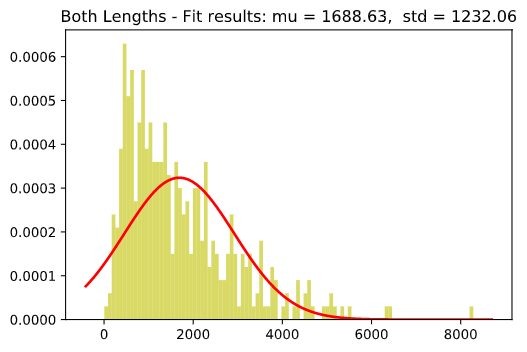
\includegraphics[scale=0.5]{Images/Lengths-Histogram.png}
    \caption{Histogram of length of mouse events for turker and lab data.}
    \label{fig:normaldis}
\end{figure}

Figure \ref{fig:normaldis} shows a the frequency of different mouse events lengths.
In red we can see a positively skewed normal distribution which matches the distribution fairly well.
When determining n for the new sequence data, we will sample from a gaussian distribution with a mean of 1688 and a standard deviation of 1232.
This should generate a realistic distribution of lengths, and when combined with the trained HMM model, a realistic sequence of data.

% TODO: model with the actual distribution, such as a log normal, or find a way to deal with the negative values.


\subsubsection{Revisiting methods}

With the generated lab study data we can now revisited some of the methods that failed due to imbalanced classes.
With the naive bayes of counts of different mouse targets, there was little improvement, with an accuracy and f1 score of 49\% and 46\% respectively.
However there was a big improvement when the bi-grams of events were fed into the model.
The accuracy and f1 scores increased to 94\%, a dramatic increase.
This shows that there is enough difference in the data for a classification algorithm to distinguish the points. 

\section{Results}
% talk about results
% Should I talk about all the results, or just the end results that I feel are conclusive.

Now the real aim of the project can begin, attempting to classify users as paying attention or not.
We will take the 2 HMMs and feed it in the existing mouse data.
This will tell use the likelihood that that sequence of mouse events belongs to each class.
If there are any points that appear to be outliers, then we can say that they were doing something differently to the majority of the turkers.
If the same outlier also has a higher likelihood of belonging to the HMM trained on lab data then we can say that that outlier sample appears to belong to the wrong group.
Or at least that outlier is doing something different to their peers, which may be a higher level of attention given to the task. 


\subsection{Table or graph of results}
% Plot histogram of likelihoods for both classes on both HMM models.
% Examine outliers.
% TODO: Idea, use a 2d histogram, or scatter plot lab likelihood against turk likelihood.


\begin{figure}[ht!]
    \centering
    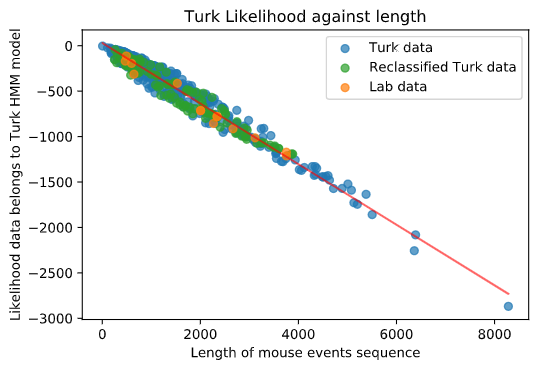
\includegraphics[scale=0.5]{Images/Turk-Lab-Liklihoods.png}
    \caption{The comparative likelihoods of users classifiers with the Turk and Lab data. }
    \label{fig:TurkLabLikli}
\end{figure}

Figure \ref{fig:TurkLabLikli} shows how closely each users mouse sequences match the different HMM models.

The model likelihoods are the the log likelihoods that each user belongs to the lab or turk models. 
One way of attempting to classify users is to identify any users with a higher lab likelihood as being more similar to a lab user than a turk user
, however all the points have a higher lab likelihood than turk likelihood shown by the black line y=x.

% An alternative solution is to plot a regression line of the lab users likelihoods (shown in orange). 
% We can see that the lab data points form an almost straight line. 
% Any points above this line have a higher likelihood of being a lab user or a lower likelihood of being a turk user than the actual lab data. 
% Thus this regression line forms a sort of pareto frontier, with points above it a more feasible choice of lab-like data than points beneath it.  


\begin{figure}[ht!]
    \centering
    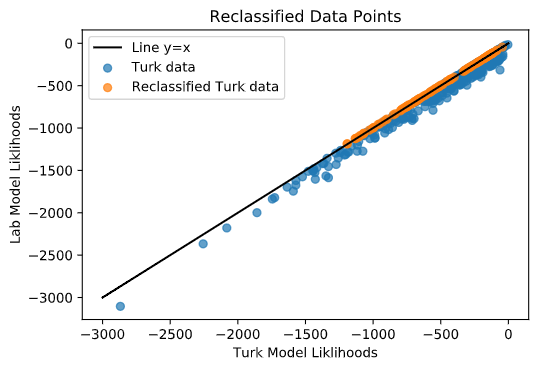
\includegraphics[scale=0.5]{Images/Reclassified-Data.png}
    \caption{Plot showing the turk users that have been reclassified as behaving more like lab users. }
    \label{fig:Reclassified}
\end{figure}

Figure \ref{fig:Reclassified} shows which of the turk users are more similar to the lab users
, than other turk users. 
This plot shows the same datapoints and axis
, but the points above the line are recoloured yellow to show their difference from the actual lab data (green) and normal turk data (purple). 
120 of the 461 (26\%) turk users are above this threshold. 
Which seems like a reasonable percentage of the population to be paying attention. 
% TODO see if I can find any references that say how many turkers/anyone pay attention at a given time.
The exact distribution of these points change based on the initial random state when training the model.

\subsection{Likelihood length correlation}

Examination of the extreme points with the highest and lowest likelihoods revealed a potential correlation likelihoods and length of mouse events sequences.
I decided to plot this data to understand if there was actually a link between these features.

\begin{figure}[h!]
    \centering
    \begin{subfigure}[c]{0.4\linewidth}
        \centering
        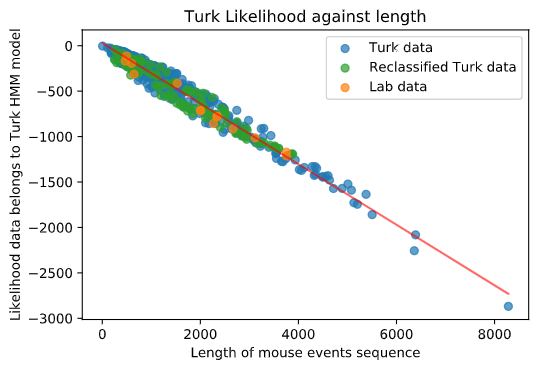
\includegraphics[scale=0.4]{Images/Turk-Liklihood-Length.png}
        \caption{Turk HMM Model}
    \end{subfigure}    
    \hfill
    \begin{subfigure}[c]{0.4\linewidth}
        \centering
        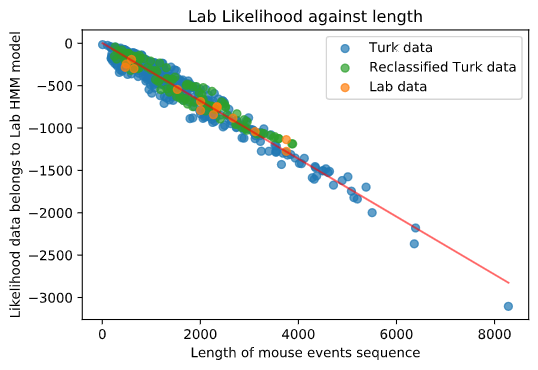
\includegraphics[scale=0.4]{Images/Lab-Liklihood-Length.png}
        \caption{Lab HMM Model}
    \end{subfigure}  
    \caption{Plots showing correlation between likelihood of different models and the length of mouse events.}
    \label{fig:liklihoodlengths}
\end{figure}

Figure \ref{fig:liklihoodlengths} show that the log likelihood from both models and length of a users mouse sequence are highly inversely correlated. 
The Lab model likelihood and length have a correlation of -0.982, and similarly the Turk model has a correlation of -0.976.
A value less than $-0.7$ would indicate a strong negative correlation, therefore Figure ~\ref{fig:liklihoodlengths} shows an extremely strong negative correlation \cite{mindrila2017scatterplots}.
Such a strong correlation could indicate the models are doing nothing, other that looking at the length of a sequence.
However looking at the reclassified Turk data we can see that there doesn't appear to be any correlation between length, and whether the data has been reclassified.
Therefore such a strong correlation between the length and likelihood is of no concern. 

\begin{figure}[ht!]
    \centering
    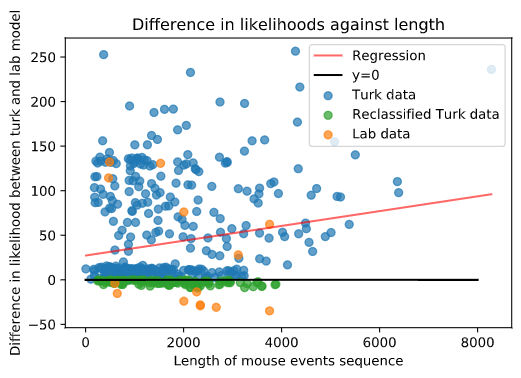
\includegraphics[scale=0.4]{Images/Difference-Liklihood-Length.png}
    \caption{Plot showing difference in likelihood between the models against length of mouse events sequence. }
    \label{fig:diffliklihoodlengths}
\end{figure}

Figure ~\ref{fig:diffliklihoodlengths} removes the concern that length of mouse events sequence is the only feature being used in the models.
The difference in likelihoods and length of mouse events sequence has a correlation of $0.176$, meaning the relationship between the features is non-existant.

\section{Conclusion}

To evaluate the results I would not be too confident in my findings.
The data was incorrectly labelled for the task I wanted to perform.
Additionally the data was heavily imbalanced.
All of the conclusions I have made from the lab data are relying on only a handful (13 maybe) of datapoints which is not statistically significant.
Additionally there was not a lot of data from the other class of online data either.
Typically data science and machine learning uses big data, where as this project used only 400ish records in total which came to only 500mb of data (MAYBE).
Any bias in any of these original samples will be magnified as this was used to classify more points, which would again spread this bias.
This would become a self fulfilling prophecy as more similar points would be labelled and spread the belief.

Any concern that the models have learned of a simple feature such as sequence event has been disproven
, showing the reclassification algorithm has nonesuch simple relationship.

Biggest flaw of the project is the first assumption, that the lab people were all paying attention.
While they were monitored and we can be sure they were not distracted by phones or televisions, many of them may have 'zoned out' and not have been given it their full effort and attention.

\section{Future work}
It would be interesting to see if any of the methods here would reveal anything interesting in other datasets.
A kaggle crowdflower dataset seems like an idea candidate and I would be interested if we could determine if any of these users were paying attention. 

\printbibliography

\end{document}